
%%% Local Variables:
%%% mode: latex
%%% TeX-master: t
%%% End:

\chapter{引言}
\label{chap:intro}

随着互联网与云计算的发展,越来越多的应用从本地迁移到云端,并涌现出大量新兴的互联网应用,
承载这些应用的数据中心成为了如同电力系统一样的社会基础设施。
与此同时,现代数据中心正在面临着权衡资源利用率与应用服务质量的挑战:
从应用开发者角度,服务质量是第一位的,因为它直接关系到用户体验与其收益,
由于互联网应用负载的波动性,开发人员通常会为自己的应用过量分配资源以满足峰值时的负载需求,
这造成了数据中心6\%$\sim$12\%极低的利用率;
而对于数据中心运维人员,资源利用率直接反映其运维成本,虽然将不同应用混合部署到同一台服务器,
充分利用空闲时段的服务器资源可以有效提高数据中心利用率,
但多应用混合部署引入的软硬件资源共享会造成应用间无管理的资源竞争,
使得应用性能出现不可预测的波动,进而影响应用的服务质量。
由上可知,如何权衡数据中心资源利用率与应用服务质量是当前数据中心亟待解决的重要问题。

%%% ---- begin cut from chap02, to be merged ----
%%互联网应用如电子邮件、搜索、网络购物、社交网络、在线视频、网络地图等,
%%已经成为人们生活的一部分。
%%这些应用往往要为上亿用户服务,意味着互联网应用已变成如电力一样的社会公共服务,
%%而支撑拥有海量用户互联网应用的数据中心也成为如同发电厂一样的社会核心基础设施。
%%
%%长尾延迟(Tail Latency)问题在数据中心中受到越来越多的关注,
%%造成长尾延迟的原因有很多,其中最为重要的原因就是资源共享带来的干扰。
%%由于缺少行之有效的方案对干扰进行控制,目前典型的数据中心都使用基于隔离的方案来减小干扰,
%%该方案虽然有效缓解了长尾延迟,但它也带来了资源利用率过低的问题,
%%现有商用数据中心的资源利用率普遍只有6\%$\sim$12\%左右,造成极大的浪费。
%%如何解决服务质量与资源利用率冲突的问题是当前业界面临的重大挑战。

本章内容安排如下:
首先介绍新计算模式对数据中心的挑战,
然后讨论现有数据中心技术的局限性,即服务质量与资源利率冲突的原因,
进而引出本文的研究动机与解决方案,
最后介绍本文的主要贡献和组织结构。

%服务质量(QoS)与资源利用率是数据中心运营时需要考虑的2个重要指标,前者严重影响用户
%体验,而后者直接与数据中心的运营成本相关。然而现有的计算机体系结构并没有为服务质量
%保障提供足够的支持,造成这2个指标在现实状况下存在冲突。为了保障用户体验,在实际系
%统部署时,会更多的考虑服务质量这一指标,造成数据中心的资源利用率严重低下,普遍只有
%10\%-30\%左右。基于这一现状,本文主要讨论如何设计一种高效的数据中心体系结构,使得
%数据中心在保障应用服务质量基础上,达到较高的资源利用率。
%
% ---- end cut ----

\section{新计算模式的挑战}

\subsection*{计算模式1:以云计算为基础的移动计算}

随着移动设备(平板电脑、智能手机)计算能力不断增强、
成本不断降低以及无线通信技术的快速发展,移动计算时代已经来临。
如表\ref{tab:ganter-sales}所示,
Gartner调研数据显示平板电脑和手机(包含智能手机和普通手机)销量不断增加,
与此同时PC销量则不断下降。
其中2016年智能手机销量将超过19亿部,
占所有个人计算设备(包括PC、平板电脑和智能手机等)77\%的销量份额。

% Gartner关于电脑与移动设备销量的统计 
\begin{table}[htb]
  \centering
  \begin{minipage}[t]{0.9\linewidth}
  \caption[全球个人计算设备市场销量统计]{全球个人计算设备市场销量统计(单位:千部)}
  \label{tab:ganter-sales}
    \begin{tabular*}{\linewidth}{lrrrrr}
      \toprule[1.5pt]
      {\heiti 设备类型} & {\heiti 2012年} & {\heiti 2013年} & {\heiti 2014年} & {\heiti 2015年} & {\heiti 2016年} \\
      \midrule[1pt]
      PC(台式机、笔记本) &   341,273 &   296,131 &   279,000 &   259,000 &   248,000 \\ 
      超级本               &     9,787 &    21,517 &    39,000 &    62,000 &    85,000 \\ 
      平板电脑             &   120,203 &   206,807 &   216,000 &   233,000 &   259,000 \\ 
      手机                 & 1,746,177 & 1,806,964 & 1,838,000 & 1,906,000 & 1,969,000 \\ 
      其他移动设备         &       --- &     2,981 &     6,000 &     9,000 &    11,000 \\
      %总计                 & 2,217,440 & 2,334,400 & 2,378,000 & 2,470,000 & 2,572,000 \\
      \bottomrule[1.5pt]
    \end{tabular*}\\[2pt]
    \footnotesize
    数据来源:Gartner,2012年(http://www.gartner.com/newsroom/id/2610015),
    2013年(http://www.gartner.com-\\/newsroom/id/2791017),
    2014-2016年(http://www.gartner.com/newsroom/id/2954317)
  \end{minipage}
\end{table}

移动计算的快速发展带来新的计算模式:
移动设备通过无线通信与运行在云计算平台的各类应用服务进行交互。
据可靠消息,目前一些主要的互联网公司(如Facebook和Baidu等)均表示,
来自移动设备的请求已占到40\%以上,并且仍在快速增长,很快将超过PC。
随着4G时代的到来,这种移动计算模式将成为未来的主流。

快速增长的移动计算需求对云计算平台的核心------数据中心带来了严峻的挑战。
这种交互式计算模式,快速的服务响应时间是衡量服务质量(Quality-of-Service,QoS)的关键指标,
是让用户满意、留住用户的关键。有研究表明,如果服务响应时间增加,公司收入就会减少。
例如,2009年微软在Bing搜索引擎上也开展实验,发现当服务响应时间增加到2000ms时,
每个用户带给企业的收益下降了4.3\%。
由于该实验对公司产生了负面影响,最终不得不被终止\cite{bing:2009}。
Amazon也发现其主页加载时间每增加100ms就会导致销售额下降1\% 。
而Google更是发现当搜索结果返回时间从0.4s增加到0.9s时,广告收入下降了20\%。

\begin{figure}
\begin{minipage}{0.48\textwidth}
  \centering
  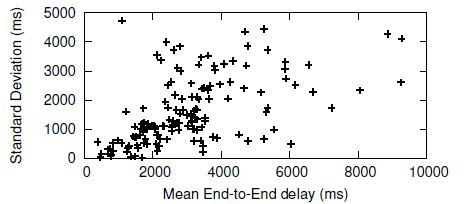
\includegraphics[height=5cm]{bg/end2end-delay}
  \caption[北美移动应用用户感知时延分布]{北美移动应用用户感知时延分布:平均延迟超过2s且具有很大的波动性}
  \label{fig:end2end-delay}
\end{minipage}\hfill
\begin{minipage}{0.48\textwidth}
  \centering
  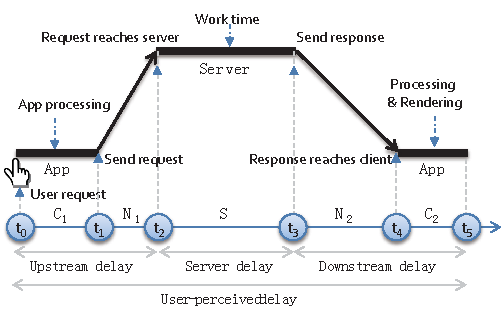
\includegraphics[height=5cm]{bg/interact-apps}
  \caption[典型交互式请求的5个阶段]{典型交互式请求的5个阶段:
    C1$\rightarrow$N1$\rightarrow$S$\rightarrow$N2$\rightarrow$C2\cite{timecard:2013}}
  \label{fig:interact-apps}
\end{minipage}
\end{figure}

移动计算的响应时间仍然存在很大的提升空间。
微软公司实验数据(图\ref{fig:end2end-delay})表明在北美网络环境下,
交互式移动设备的平均时延超过2s,而且存在较大的波动性。
图\ref{fig:interact-apps}显示典型移动交互式应用的用户请求时延分为5个阶段,
最近研究\cite{timecard:2013}表明其中数据中心服务器的处理时延S约为1.2s,占60\%。
随着4G网络的普及,数据中心面临更大规模用户数据的处理请求。
因此,如何快速处理和及时响应移动计算请求将成为数据中心设计的核心目标之一。


\subsection*{计算模式2:面向大数据处理的实时计算}

大数据时代的到来使大数据处理架构受到越来越多的关注。
2013年底中国计算机学会(CCF)大数据专家委员会发布的
《2014年大数据发展趋势十大预测》报告中,
来自学术界、产业界、海外、跨界特邀和政府的122位专家们普遍认为,
Hadoop/MapReduce框架一统天下的模式将被打破,
而实时流计算、分布式内存计算、图计算框架等将并存。

\begin{figure}[H]
  \centering
  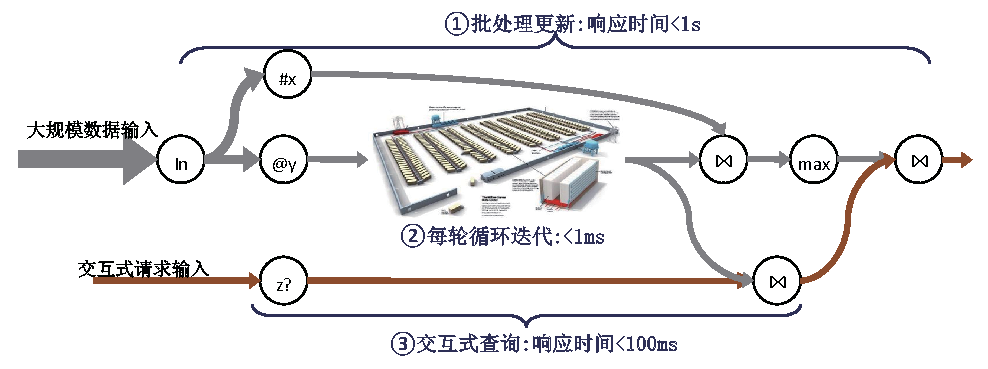
\includegraphics[height=6cm]{bg/batch-apps}
  \caption{典型的3类大数据处理需求以及相应的响应时间要求}
  \label{fig:batch-apps}
\end{figure}


大数据处理对数据中心和处理架构提出新的挑战,
图\ref{fig:batch-apps}显示了典型的大数据处理需求:
首先需要支持数据的批处理更新模式(<1s);
其次数据处理会分解为多次迭代计算(<1ms);
再次还要支持实时计算模式,处理多用户的交互式查询请求(<100ms);
而这些处理所需要的数据存放在同一个数据中心。
搜索引擎是一个典型的例子,既需要对大规模网页进行内容处理,迭代计算页面的PageRank,
还需要处理大量用户的关键字查询请求。

尽管大数据处理希望能将各种处理集成在一个处理架构上,然后部署在一个数据中心,
但如果实时计算与企业营收相关,比如搜索引擎、在线购物等在线服务应用,
那么正如微软Bing实验所示,这些面向在线服务应用的实时计算的服务质量就非常关键
(以下用``在线应用''代表``实时计算'')。
为了保障在线应用的服务质量,
主流互联网企业一般将在线应用与大规模批处理作业分别部署到不同的数据中心,
以减少批处理作业对在线应用的干扰。
但由于用户查询请求数量具有显著的随时间变化的波动性,
这种分离作业、单独部署的模式会导致在线应用数据中心的资源平均利用率很低。
如图\ref{fig:google-util-2013}所示,Google的2类数据中心CPU利用率相差达2.5倍,
在线应用数据中心资源利用率仍有很大提升空间。


%% 典型的数据中心一般有5~10万台服务器组成,建设与运行维护成本往往高达几十亿人民
%% 币。然而出于保障应用服务质量的原因,现有数据中心只能维持较低的资源利用率,导致大量
%% 资源浪费。因此,本项目总体研究目标为如何设计高效通用数据中心体系结构:``通用''表
%% 示数据中心可同时运行各种不同类型应用;``高效''表示数据中心能在保障延迟敏感应用的服
%% 务质量基础上,达到较高的资源利用率(CPU利用率>60\%)。
%% 
%% 典型的数据中心一般有5~10万台中低端服务器组成,这些服务器通过内部网络互连,一起协同
%% 运行互联网应用为海量用户服务。因为这类数据中心规模很大,往往部署在大型仓库级别的机
%% 房,从应用角度来看就如同一台计算机,因此也被称为
%% ``仓库级计算机(Warehouse-Scale Computer)'' \cite{WSC}。
%% 国内外著名的互联网公司往往拥有多个数据中心,服务器数量达到数十万甚
%% 至上百万台。例如,谷歌(Google)的数据中心服务器数量已经超过百万台为全球用户提供
%% 搜索、邮件、地图等服务[2];亚马逊(Amazon)仅EC2就部署了约50万台服务器提供云计算服
%% 务[3];据可靠消息,国内腾讯公司也拥有约30万服务器为用户提供各种互联网服务。
%% 
%% 尽管目前互联网企业的数据中心已经颇具规模,但一个趋势是未来数据中心还将持续发展。一
%% 方面互联网用户数量仍在不断增长,目前全球已有24亿网络用户,但很多机构预测未来全球还
%% 将新增30亿网民融入到互联网[4],这会对数据中心的数量和规模都提出更多需求。另一方面快
%% 速发展的移动终端已超越个人计算机(PC),成为终端计算设备的主流。由于移动设备性能相对
%% 较低、存储容量较小,将计算与存储转移到数据中心的需求也变得越来越强烈。因此数据中心作
%% 为基础设施也会日益重要。


\section{现有数据中心技术的局限性}

通过上述分析可知,移动计算与实时计算均对快速响应用户请求提出了强烈的需求。
而当前数据中心为了保障用户请求的服务质量,
不得不通过采用牺牲资源利用率、保留过量资源的方式。
以Google的数据中心为例,
图\ref{fig:google-util-2006}显示了2006年Google数据中心平均CPU利用率为30\%左右。
但到2013年,虽然Google将数据中心分为了2类,并且批处理数据中心已经能达到75\%的CPU利用率,
但在线应用数据中心仍停留在30\%。
Google的数据中心技术一直处于领先地位,
与之相比,国内一些主流互联网企业在线应用数据中心CPU利用率一般都低于20\%,
有的甚至低于10\%,仍然存在很大的提升空间。

% Google数据中心利用率 
\begin{figure}
\begin{minipage}{0.57\textwidth}
  \centering
  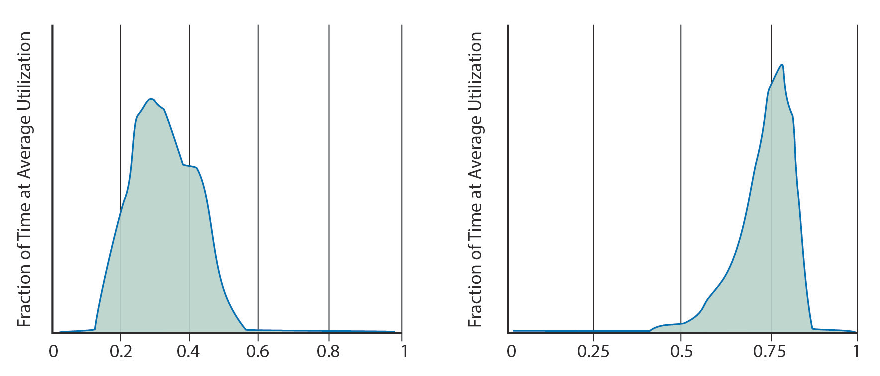
\includegraphics[height=4cm]{bg/google-util-2013}
  \caption[Google数据中心CPU利用率分布(2013年)]
    {Google数据显示2013年1至3月在线应用数据中心CPU利用率平均只有30\%(左图),
     而批处理作业数据中心则能达到75\%的利用率(2个数据中心均为2万台服务器)\cite{barroso_datacenter_2013}}
  \label{fig:google-util-2013}
\end{minipage}\hfill
\begin{minipage}{0.39\textwidth}
  \centering
  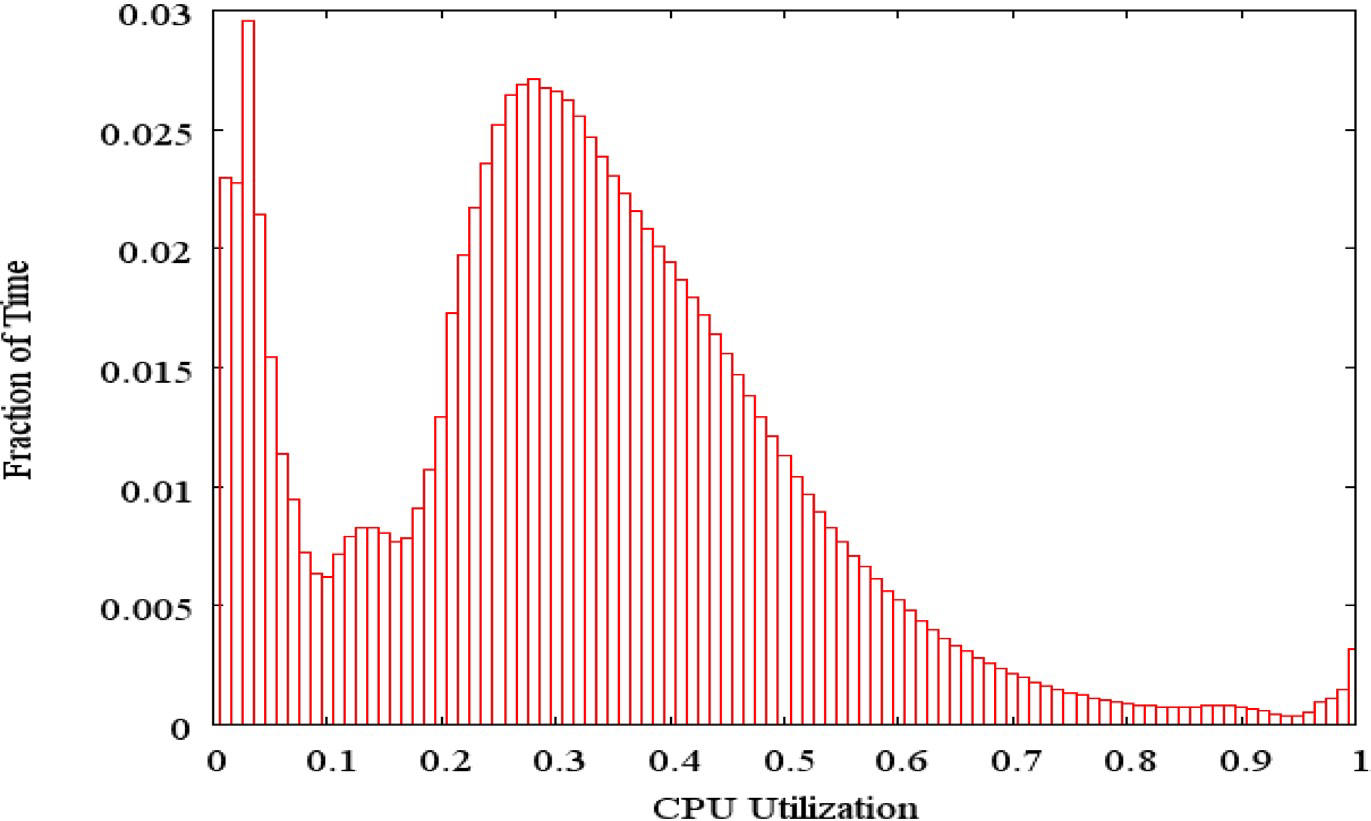
\includegraphics[height=3.5cm]{bg/google-util-2006}
  \caption[Google数据中心CPU利用率分布(2006年)]
    {Google在2006年数据中心(5000台服务器)6个月的CPU利用率分布\cite{barroso_datacenter_2009}}
  \label{fig:google-util-2006}
\end{minipage}
\end{figure}

尽管在线数据中心资源利用率只有30\%,但Google已经观察到严峻的长尾延迟现象:
最慢的1\%$\sim$10\%请求处理时间远大于所有请求的平均响应时间。
如图\ref{fig:google-resptime-dist}所示,Google某后台服务延迟响应时间平均仅为5$\sim$6ms,
但是却有相当一部分请求响应时间超过了100ms\cite{Krushevskaja:2013}。
而长尾延迟现象在数据中心环境下会被更进一步放大,
因为1个用户请求需要几百上千台服务器共同完成,只要有1台服务器的处理速度受到干扰,
就会导致整个请求的处理时间增加。
Google的Jeff Dean在2012年Berkeley的报告\cite{dean_achieving_2012}中
就指出了长尾现象的严重性:假设1台机器处理请求的平均响应时间为1ms,
有1\%的请求为长尾处理时间会大于1s(99th-Percentile);
如果1个请求需要由100个这样的节点一起处理,那么就会出现63\%的请求响应时间大于1s
(如图\ref{fig:long-tail-amplify}所示)。

造成在线应用数据中心资源利用率低和长尾延迟现象的核心原因是,
现有数据中心技术无法在多应用混合运行时消除应用间干扰,以实现不同应用之间的性能隔离。
Google的Jeff Dean与Luiz Barroso在2013年2月的《Communication of the ACM》上撰文
``The Tail at Scale''\cite{dean_tail_2013}分析确认导致长尾延迟的首要原因就是资源共享,
包括体系结构层次的CPU核、Cache、访存带宽、网络带宽等,而干扰不仅来自应用,
还会来自系统软件层次的后台守护作业、监控作业、共享文件系统等。
Google在分布式架构和软件层次采用了多种缓解长尾延迟的技术,
包括操作系统容器隔离技术\cite{cgroup}、应用优先级管理\cite{Reiss_googletrace_2012}、
备份请求\cite{dean_achieving_2012}、同步后台管理进程\cite{dean_achieving_2012}等,
取得了一定的效果,但却无法消除硬件体系结构层次上的应用之间的干扰,
导致仍然会出现图\ref{fig:google-resptime-dist}这样的长尾延迟。

\begin{figure}
\begin{minipage}{0.52\textwidth}
  \centering
  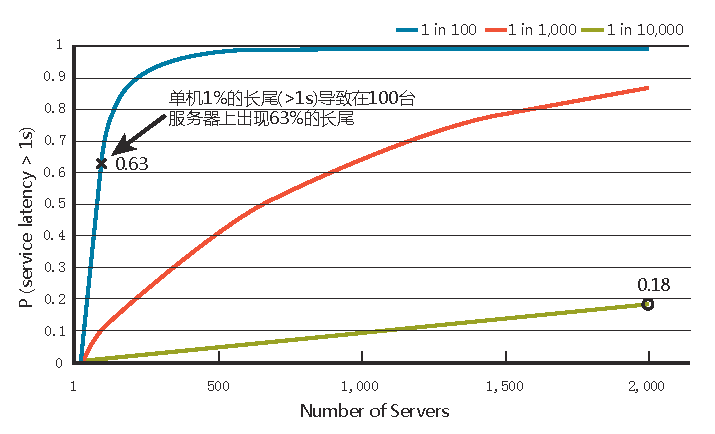
\includegraphics[width=\textwidth]{bg/long-tail-amplify}
  \caption[长尾延迟放大效应]{长尾延迟放大效应\cite{dean_tail_2013}}
  \label{fig:long-tail-amplify}
\end{minipage}
\begin{minipage}{0.44\textwidth}
  \centering
  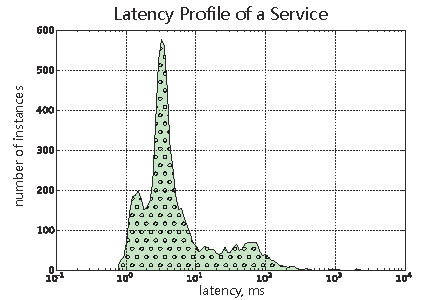
\includegraphics[width=\textwidth]{bg/google-resptime-dist}
  \caption[Google某后台服务的响应时间分布]{Google某后台服务的响应时间分布\cite{Krushevskaja:2013}}
  \label{fig:google-resptime-dist}
\end{minipage}\hfill
\end{figure}

因此,现有数据中心处于``无管理的资源共享''状态,
这导致出现资源利用率与应用服务质量之间的矛盾:
一方面通过多个应用同时在数据中心部署实现资源共享能有效提高资源利用率,
但另一方面多个应用共享资源又会出现相互干扰严重影响应用的服务质量。
因此,目前企业不得不采用预留额外资源以保障延迟敏感的在线应用服务质量,
这导致很低的数据中心利用率。
而且随着多核技术的发展,单个服务器内的资源越来越多,
其上混合部署的应用数目也在不断增加,更会加剧这种矛盾。


\section{研究动机}

当前主要从3个角度应对上述问题:
其一是通过上层软件机制实现干扰容忍,在应用层保障服务质量,
如Google提出的Hedged Requests和Tied Requests方案\cite{dean_tail_2013},
通过向多个副本发送请求,并选择最快返回的结果以达到干扰容忍的目的;
R. Kapoor等人在文章\cite{Kapoor:2012:Chronos}中提出了Chronos架构,
以降低数据中心应用的长尾延迟;
另外一些工作\cite{timecard:2013, d2p:2014}尝试记录单个请求延迟在每个环节处理时间,
然后在分布式处理框架中传播,基于这些传播的信息来进行请求的处理与调度。
其二是在作业调度层次,通过profile的方式预测应用混合后的干扰情况,
将相互之间干扰较小的应用部署到同一台服务器\cite{mars_bubble-up:_2011, kambadur_measuring_2012}。
其三是提供一个良好的隔离环境,降低由资源竞争所产生的应用间干扰,
可以在各个层次实现隔离,
如数据中心作业调度层\cite{Hindman:2011:Mesos, Schwarzkopf_omega_2013, borg:2015}、
操作系统\cite{cgroup, lin_gaining_2008, tam_managing_2007, liu_software_2012, Liu:2014:ISCA}、
虚拟化层\cite{Xu:2013:Bobtail:, Xu:2013:SMALL}、
硬件\cite{kasture_ubik:_2014, sanchez_vantage:_2011, sanchez_zcache:_2010, qureshi_utility-based_2006, muralidhara_reducing_2011}等。


其中前2种方案在实施时需要对目标应用具有非常深入的理解:
方案1需要对应用架构与实现细节进行修改,以达到应用层干扰容忍的目的;
方案2虽然无需对应用进行修改,但需要对应用的资源占用以及不同应用之间的干扰状况进行分析,
才能得到最优的调度方案。
当应用数量不多且有条件进行以上所述的分析或修改,通过精细的应用架构设计与调度机制,
可以有效的解决前文所提到的资源利用率与服务质量相冲突的问题。
但在现实数据中心特别是云计算数据中心内,以上假设并不成立。

首先,数据中心内通常会运行大量的应用,
如Google的数据\cite{Reiss_googletrace_2012}表明其数据中心在2个月内累计运行超过2,000,000个应用,
无论是改造这些应用或是对应用之间的干扰行为进行分析都是不可行的。
即使只对部分关键的应用进行改造使其适应干扰环境,
云计算环境下的``吵闹的邻居(Noisy Neighbors)''也会使这些努力的结效果大打折扣。

其次,调度方案无法解决短时运行的干扰应用对其他正常应用带来的影响,特别是随着DevOps的兴起,
由于开发调试与线上部署是不断迭代进行的,调试过程中所引入的短时干扰应用数量大大增加,
Google的数据\cite{Reiss_googletrace_2012}发现大量的小于6分钟的应用都是来自于这些调试应用。
当调度器发现干扰并准备采取调度措施时干扰应用可能已经结束,同时新的干扰应用又开始运行,并带来新的干扰。

对于第3种隔离方案,
单纯软件层次的隔离只能做到较粗粒度的资源管理,实现的效果有限;
同时应用的不同特征造成资源竞争点是分布在整个软件栈中,
因此只能根据实际场景做针对性的优化;
再次,在如此复杂的软件栈中找到真正的资源竞争点需要大量的时间与精力,
这同样不能满足云计算的场景下应用多样与快速部署的需求。
除了软件栈上的共享,混合部署的应用在硬件层次上也存在大量的共享,
如共享末级缓存、内存控制器、I/O等,
上文所提到的这些研究专注于如何在这些共享硬件上提供隔离功能,
但这些研究大都只关注于一种类型的资源,而且是针对特定的场景,
因此缺少灵活的软件编程接口,不能适用于通用的计算场景。

综上可知,
现有的3种方案都不能很好的解决当前云计算数据中心中遇到的资源利用率与服务质量矛盾的问题,
该问题的本质是为应用提供区分化服务,
而如何解决目前计算机系统的软硬件资源的无管理共享状态是实现区分化服务的关键。
现有研究在一定程度上能够解决软件层次的共享管理问题,
但无管理的硬件共享使得该问题并没有被完全解决。
造成这一现状的原因是目前的计算机体系结构在设计时并没有考虑到多应用共享场景,
其指令集抽象不足以将上层应用需求传递到下层硬件,
在不能区分应用需求的前提下很难做到区分化服务。
软件层次已有很多方案可以用于区分不同应用,如操作系统级的进程PID或cgroup,
或更细粒度的应用级标签\cite{timecard:2013,d2p:2014, mesnier_differentiated_2011, thereska_ioflow:_2013}。
硬件层次也需要一种应用需求传递机制。
% -- removed by advisor
%%正如``21st Century Computer Architecture''白皮书中所提出的:
%%
%%\begin{quotation} 
%%\emph{\textbf{Better Interfaces for High-Level Information.}
%%Current ISAs fail to provide an efficient means of capturing software-intent or conveying critical high-level information to the hardware.
%%For example, they have no way of specifying when a program requires energy efficiency, robust security, or a desired Quality of Service (QoS) level.
%%Instead, current hardware must try to glean some of this information on its own ......
%%\textbf{New, higher-level interfaces are needed to encapsulate and convey programmer and compiler knowledge to the hardware,}
%%resulting in major efficiency gains and valuable new functionality.}\cite{21st_architecture}
%%\end{quotation}

因此,我们需要为数据中心计算机设计一种新的体系结构,
使其能够从硬件上改变资源的``无管理共享''现状,
从体系结构上支持应用服务质量保障,
在此基础上实现数据中心资源根据应用动态管理以提高资源利用率。

\begin{figure}[t]
  \centering
  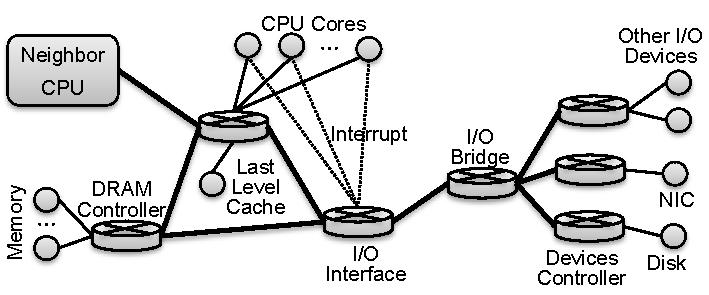
\includegraphics[height=4cm]{intro/computer-as-a-network.pdf}
  \caption[计算机内部本质是一个网络]{
    计算机内部部件之间以数据包(packet)进行通信,比如
    处理器核之间使用基于包的片上网络、
    处理器之间采用基于包的互连协议(如QPI和HT)、
    I/O设备与内存之间则通过PCI-E包进行通信。
    因此,计算机本身即可视为一个网络。}
  \label{fig:computer-as-a-network}
\end{figure}

基于以上需求,
本文提出了一种新型体系结构实现:资源按需管理可编程的体系结构PARD
(Programmable Architecture for Resourcing-on-Demand)\cite{pard:2015},
使数据中心服务器能够支持区分化服务,通过细粒度的硬件资源管理以及灵活的编程接口,
实现在保障关键应用服务质量的前提下提高服务器资源利用率的目标。
PARD体系结构的核心是基于一个重要的观察:\textbf{计算机内部本质上是一个网络}。
如图\ref{fig:computer-as-a-network}所示,
CPU核、共享缓存、内存控制器、I/O设备等可以被看做是网络节点,它们之间通过包进行通信;
除了处理请求以外,这些``网络节点''与网络中的路由器/交换机具有相似的请求转发功能。
在网络领域,如何实现端到端的服务质量保障已有大量的研究,并已形成标准。
如IETF(Internet Engineering Task Force, 互联网工程任务组)于1998年提出了区分化服务
(Differentiated Services)\cite{DiffServ}的概念,
如今区分化服务已经成为应用最广泛的服务质量保障机制之一;
软件定义网络(SDN)\cite{SDN}的出现,进一步促进了网络领域服务质量保障的发展,
其提出的控制平面与数据平面分离和集中控制的统一编程接口,为网络管理带来了极大的灵活性。
本文希望能够将网络领域的区分化服务和软件定义网络的思想应用到计算机内部的网络,
用以解决数据中心当前面临的资源利用率与应用服务质量矛盾。

然而相比在计算机网络,
在体系结构这一``内部网络''中实现区分化服务与软件定义网络的功能需要面临一些额外的挑战:

首先,网络栈是整个网络中产生数据包的唯一位置,因此可以很容易的在其中增加标签机制,
实现网络流的区分。
而在计算机中有大量不同类型的硬件部件都能够向``内部网络''发送请求,
而且这些请求的类型各不相同,
如何为这些来自于不同硬件部件、类型各异的请求增加应用标签是需要解决的第1个挑战。

其次,与网络中交换机或路由器这些只进行存储转发的网络设备不同,
计算机内各个硬件部件通常包含更为复杂的功能,
如:处理器末级缓存除了需要完成将请求转发到下层内存控制器外,
还需要决定哪些请求数据缓存在本地,以及替换哪些数据到内存控制器;
内存控制器需要进行复杂的地址映射实现将物理地址映射到DRAM芯片,
同时还需要实现调度策略以提高访存性能;其他一些I/O设备具有更为复杂的功能。
因此如何为这些不同类型的硬件部分提供一个统一的控制平面实现对硬件资源的管理是第2个挑战。

最后,在交换机或路由器中已经为管理员提供了访问和配置其控制平面的固件接口,
而在当前的计算机中并没有类似的的固件接口。
服务器中普遍配置的IPMI/BMC\cite{ipmi}提供了诸如温度监控、电源控制、
BIOS访问等有限的监控与管理功能,利用该模块如何实现硬件控制平面的管理,
以及如何为用户(管理员)提供灵活的访问与编程接口是面临的第3个挑战。

为了解决以上3个挑战,PARD体系结构的核心设计理念可以归结为以下4点:
\textbf{1)标签机制},
通过在请求源(如处理器核或具有DMA功能的I/O设备)增加标签寄存器,
使用其记录当前正在使用该部件的应用标签,
发出请求时附带该标签,并随着请求在整个计算机内部传播,实现应用区分;
\textbf{2)硬件资源的控制平面与数据平面抽象},
将共享的硬件资源抽象为控制平面与数据平面2部分,
数据平面利用标签机制提供的应用信息对请求进行区分化处理,
控制平面用于对数据平面的策略与规则进行管理,
两者通过软件可编程的方式实现硬件资源管理策略的动态调整。
\textbf{3)节点内统一资源管理},
节点内所有的控制平面通过控制平面网络连接到资源管理模块,提供对控制平面的编程接口,
实现所有共享资源的统一管理;
\textbf{4)``\emph{trigger$\Rightarrow$action}''编程方法},
一种基于动作触发的资源管理策略,实现资源实时监控和调整。

本文后续章节将讨论如何在现有体系结构上扩展以实现标签机制;
通用控制平面与数据平面的设计以及可编程机制的实现,
并包括末级缓存控制器和内存控制器中控制平面的具体设计;
基于以上2种机制实现无软件Hypervisor的全硬件支持虚拟化系统,
以及如何实现资源按需分配的区分化服务,使用模拟器对其效果进行验证。
最后在基于FPGA的原型系统中验证PARD体系结构的效果,
并对其性能与资源开销进行评估。


\section{本文主要贡献}

本文的研究思路是:
在应用数量众多、需求多样且不断变化的数据中心场景下,计算机体系结构需要重新设计,
为应用提供区分化服务、良好的性能隔离,并具备灵活的资源管理编程接口,
实现资源使用的强控制与按需分配,
才能解决数据中心资源利用率与服务质量冲突的问题。

本文的主要贡献包括:

% 可在多个层次(虚拟机、进程、线程、API、...)区分应用,实现了NoHyper功能
第一,提出``性能标签''概念,用于实现应用区分。
正如多进程技术的出现引入了虚拟地址空间抽象,
随着虚拟化、云计算与多租户使用模式的出现,
现有的虚拟地址空间抽象无法满足多租户之间的隔离需求,
一些硬件隔离技术如EPT、I/O MMU、SR-IOV等试图在现有的体系结构下支持隔离需求,
其本质则是在虚拟地址空间外增加1层额外的地址空间,但这些技术只是在功能层面上实现了隔离,
而与性能相关的部件如共享末级缓存、内存控制器等在现有体系结构下并没有实现隔离。
本文提出的性能标签抽象,使用统一标签区分不同应用,
并为计算机系统内所有请求标识应用标签,硬件不再需要通过猜测的方式区分应用,
而是通过标签机制打破目前体系结构中软硬件之间的语言鸿沟,
使得共享的硬件资源能够区分来自不同应用的请求并进行区分处理。
%可在不同层次实现应用区分,如虚拟机、进程、线程或使用API标识的数据/代码段,
%以实现不同粒度的区分化服务。
%以虚拟机粒度为例,通过标签机制以及共享硬件资源内部基于标签的划分机制,
%可将一台计算机划分为多台独立的逻辑域(Logical Domain),
%在每个逻辑域内独立运行操作系统,实现NoHyper\cite{keller_nohype:_2010}的功能。

% 表+Trigger/Action <=> 处理器方案
第二,提出可编程硬件资源共享管理方法,实现节点内硬件资源的统一管理。
通过将硬件资源抽象为``控制平面''与``数据平面'',
使用软件可编程的方式对硬件资源进行统一管理,
包括基于``控制平面''的策略可编程和``数据平面''的机制可编程。
结合性能标签实现资源管理可编程体系结构,以支持数据中心复杂多变的应用场景。

%为硬件资源共享提供配置、监控、反馈功能。
%%本文2个重要观点是:资源监控与管理结合,共享资源本地与全局协同管理结合。
%实时的监控与反馈是实现细粒度资源管理的重要前提,软件监控方案无法满足实时性的需求,
%本文提出的硬件资源共享管理方法通过在硬件上直接实现监控与反馈,实现
%提出使用通用的``控制平面''实现硬件资源的配置与监控。
%在具体实现上,通过基于表的控制平面实现通用的硬件资源管理接口,
%使用基于处理器的数据平面实现硬件请求的灵活控制,
%为计算机系统实现硬件资源可管理提供支持。

第三,提出可编程体系结构硬件资源管理的软件接口,实现本地资源的灵活管理。
本文利用Linux的sysfs机制,在集中式的资源管理模块中将``控制平面''和``数据平面''抽象为文件,
为用户提供基于文件的硬件资源编程接口。
同时提出了``\emph{trigger$\Rightarrow$action}''机制实现硬件资源的实时监控与反馈调节,
以及不同资源之间的协同管理。

%通过以上硬件资源共享管理方法,将更多硬件的信息
%控制平面构成了计算机系统内硬件资源管理的基本单元,由于硬件资源之间具有关联性,
%需要进行全局统筹管理。
%本文通过使用控制面网络将节点内所有的控制平面连接到集中式的资源管理模块,
%对硬件共享资源进行协同管理。

以上3点贡献已在PARD的模拟器及FPGA原型系统中实现。
模拟器原型是基于gem5\cite{binkert_gem5_2011}实现的全系统时钟精确模拟器,
增加或修改了大约24,118行C++/Python代码,该模拟器已在LGPL协议下开源
\footnote{PARD-gem5模拟器开源地址https://github.com/fsg-ict/PARD-gem5}。
FPGA原型系统基于MicroBlaze系统在Xilinx VC709开发板实现并完成验证,
系统运行在133.33MHz频率,包含4个处理器核。
这2个原型系统可以作为后续相关研究的参考平台。


\section{论文组织结构}

\begin{figure}[htb]
  \centering
  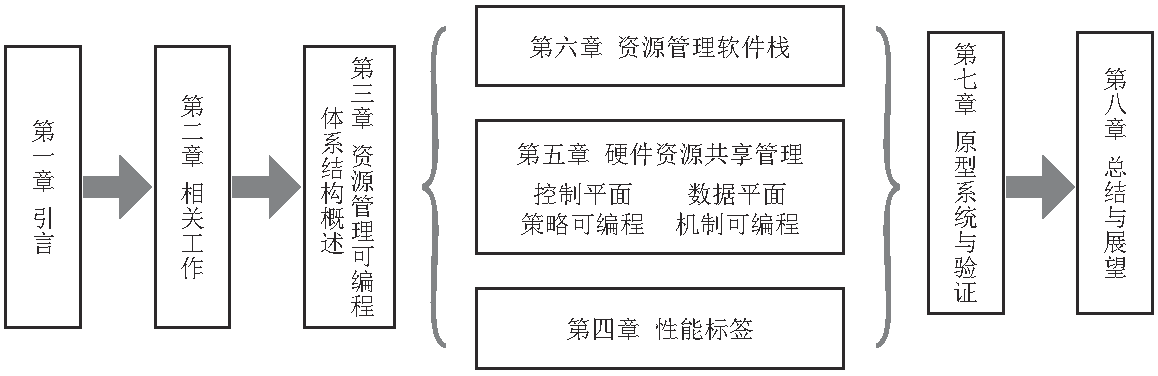
\includegraphics[width=\textwidth]{intro/thesis-structure}
  \caption{本文内容与组织结构}
  \label{fig:thesis-structure}
\end{figure}

本文共分八章,组织结构如图\ref{fig:thesis-structure}所示。

第二章介绍数据中心面临的资源利用率与服务质量冲突问题的挑战,
然后讨论现有数据中心技术的局限性,
并介绍解决该问题的现有研究。

第三章介绍PARD体系结构与关键特性,
并讨论如何利用PARD所提供的特性解决应用服务质量与资源利用率相冲突的问题。

第四章介绍PARD体系结构的基础:性能标签机制,
讨论在现有体系结构下实现性能标签需要解决的关键问题,
并在模拟器上通过利用性能标签实现无软件Hypervisor支持的全硬件虚拟化功能。

第五章讨论硬件共享资源的管理方法,包括硬件资源的控制平面/数据平面抽象,
同时以共享末级缓存和内存控制器为例,讨论控制平面与数据平面的设计,
并通过模拟的方式验证该方案的有效性。

第六章介绍资源管理软件栈的设计,包含节点内资源抽象与编程接口,
并讨论如何将PARD集成到现有的数据中心管理系统中(以Mesos\cite{Hindman:2011:Mesos}为例)。

第七章基于前四章的设计给出本文资源管理可编程体系结构的FPGA原型系统实现,
并对原型系统各部分功能的正确性、性能与开销进行评测。

第八章总结全文并介绍未来可能的研究工作。

